\documentclass[12pt]{article}
\usepackage{mathematics}

\begin{document}

\section*{Fall 2005 - Problem sets}

\subsection*{}

\subsubsection{}
\begin{mdframed}
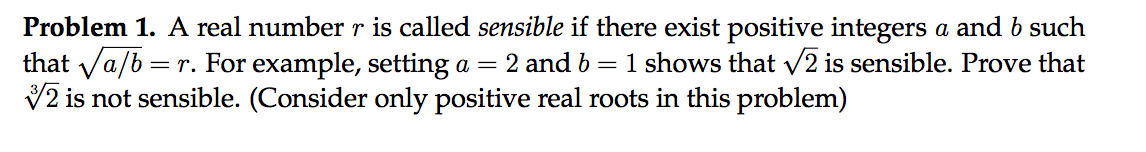
\includegraphics[width=400pt]{img/MIT-math-for-cs-2005-set-1-1.png}
\end{mdframed}


\begin{claim*}
  There does not exist $a, b \in \N$ such that $\sqrt{a/b} = \sqrt[3]{2}$.
\end{claim*}

\begin{proof}~\\
  Suppose for a contradiction that there exist $a, b \in \N$ such that $\sqrt{a/b} = \sqrt[3]{2}$,
  where $a$ and $b$ are coprime (aka mutually prime; have no common factor).

  Then $a/b = 2^{2/3}$, therefore $a^3 = 4b^3$. Therefore $a^3$ is even. Therefore $a$ is even.

  Let $a = 2c$. Then $8c^3 = 4b^3$, so $b^3$ is even. Therefore $b$ is even.

  Therefore both $a$ and $b$ are even, which is a contradiction proving the claim. \checkmark
\end{proof}

\newpage
\subsubsection{}
\begin{mdframed}
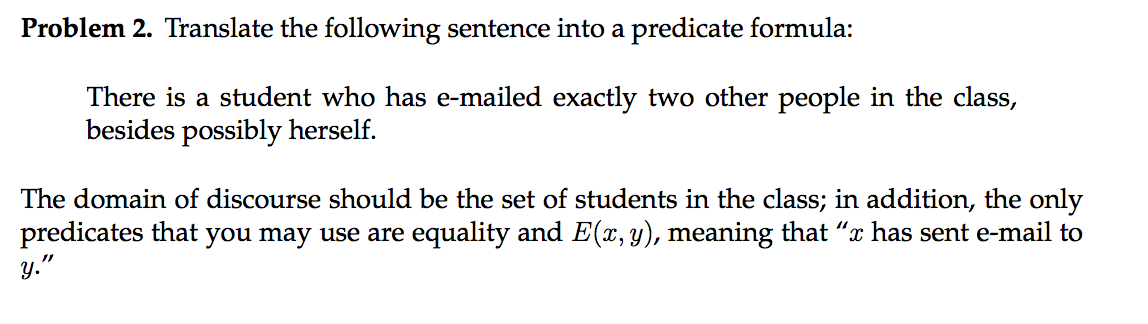
\includegraphics[width=400pt]{img/MIT-math-for-cs-2005-set-1-2.png}
\end{mdframed}

Let $X$ be the set of students in the class.

\begin{align*}
  \exists x \exists y \exists z.
  &\Big(y \neq x \land E(x, y)\Big) \land\\
  &\Big(z \neq x \land z \neq y \land E(x, z)\Big) \land\\
  &\Big(E(x, a) \rightarrow a = x \lor a = y \lor a = z\Big)
\end{align*}

\subsubsection*{}
The domain of discourse is the nonnegative integers, $\N$.

First we define the $>$ relation:
\begin{align*}
  x > y \iff \neg\exists a. y + a = x
\end{align*}

\begin{enumerate}

\item $n$ is the sum of three perfect squares.
  \begin{align*}
    \exists n ~\exists a ~\exists b ~\exists c. ~n = aa + bb + cc.
  \end{align*}

\item $x > 1$\\
  Define $x = 1$ as $\forall y. yx = y$.
  \begin{align*}
    \exists y. y = 1 \land x > y
  \end{align*}

\item $n$ is prime
  \begin{align*}
    \text{isprime}(n) := n > 1 \land \neg\Big(\exists a ~\exists b.
    \Big(
    &ab = n ~\land \\
    &a + a \neq a \land aa \neq a ~\land \\  % a \neq 0 and a \neq 1
    &b + b \neq b \land bb \neq b\Big)\Big)  % b \neq 0 and b \neq 1
  \end{align*}

\item $n$ is a product of two distinct primes
  \begin{align*}
    \exists n ~ \exists a ~ \exists b. \Big(n = ab \land a \neq b \land \text{prime}(a) \land \text{prime}(b)\Big)
  \end{align*}

\item (Goldbach conjecture) Every even natural number $n > 2$ can be expressed as the sum of two
  primes.\\
  Define $x = 2$ as $\forall y. xy = 2y$.\\
  Define $x > 2$ as $\exists y. y = 2 \land x > y$.
  \begin{align*}
    \forall n. ~ n > 2 \rightarrow \exists a ~\exists b. \text{prime}(a) \land \text{prime}(b) \land a + b = n.
  \end{align*}

\item (Bertrand's Postulate) If $n > 1$, then there is always at least one prime $p$ such that
  $n < p < 2n$.
  \begin{align*}
    n > 1 \rightarrow \exists p. ~p > n \land 2n > p.
  \end{align*}

\end{enumerate}

\begin{mdframed}
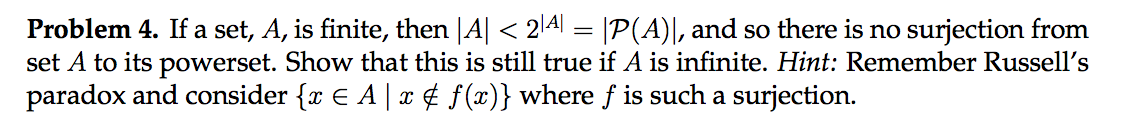
\includegraphics[width=400pt]{img/MIT-math-for-cs-2005-set-1-4.png}
\end{mdframed}

\begin{proof}~\\ \red{TODO}
  Let $A$ be infinite and suppose that $f:A \to \mc P(A)$ is a surjection from $A$ to its powerset.

  Then $f(x) \seq A$ for all $x \in A$.

  Consider $\{x \in A ~|~ x \notin f(x)\}$, the subset of $A$ containing precisely those elements
  $x$ which are not in their corresponding subset $f(x)$.
\end{proof}

\begin{mdframed}
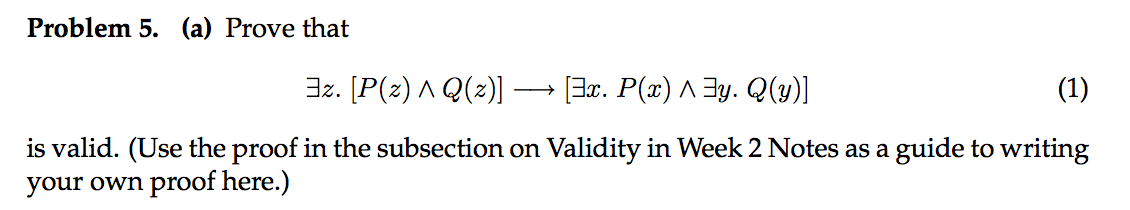
\includegraphics[width=400pt]{img/MIT-math-for-cs-2005-set-1-5.png}
\end{mdframed}
Let $D$ be the domain of the variables and let $P$ and $Q$ be arbitrary predicates on $D$. From the
LHS we know that there exists $d \in D$ such that both $P(d)$ and $Q(d)$. Therefore RHS.e

\begin{mdframed}
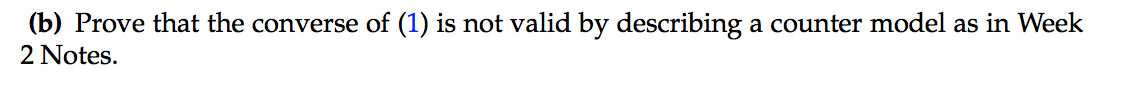
\includegraphics[width=400pt]{img/MIT-math-for-cs-2005-set-1-5-b.png}
\end{mdframed}
The converse of (1) is
\begin{align*}
  [\exists x. P(x) \land \exists y. Q(y)] \rightarrow \exists z. [P(z) \land Q(z)].
\end{align*}

A counter model is:

$P(s) := $ proposition $s$ is true.\\
$Q(s) := $ proposition $s$ is false.


\begin{mdframed}
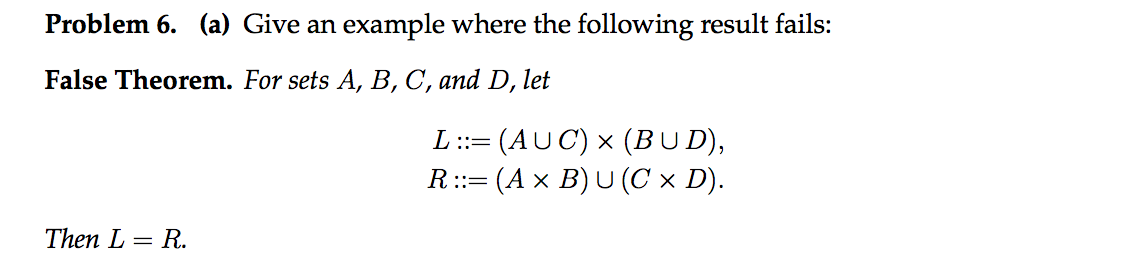
\includegraphics[width=400pt]{img/MIT-math-for-cs-2005-set-1-6-a.png}
\end{mdframed}
Let $A = \{1\}, B = \{2\}, C = \{3\}, D=\{4\}$.

Then $(1,4) \in L$ yet $(1,4) \notin R$. Therefore $L \neq R$.

\begin{mdframed}
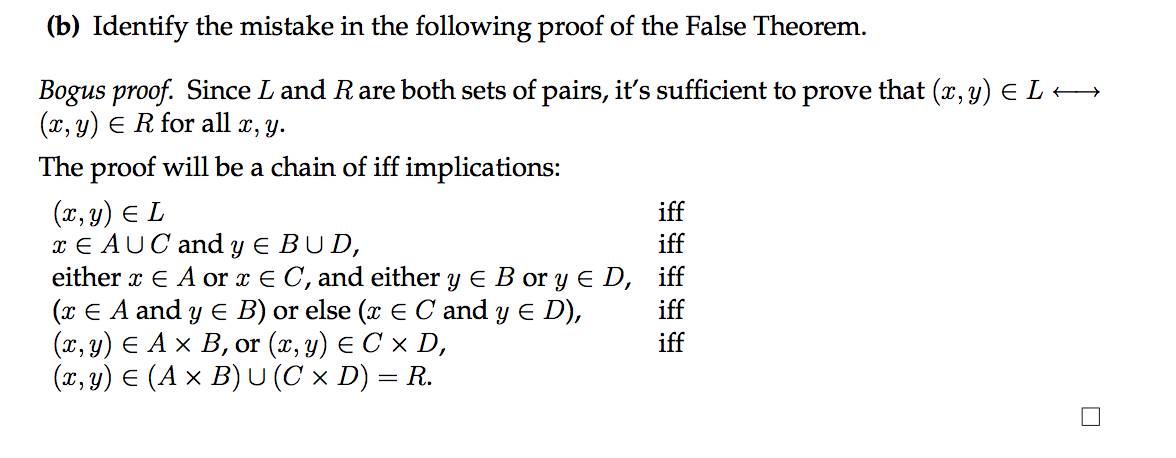
\includegraphics[width=400pt]{img/MIT-math-for-cs-2005-set-1-6-b.png}
\end{mdframed}
Mistake on 4th line: Could have ($x \in A$ and $y \in D$).
\newpage



\begin{mdframed}

\includegraphics[width=400pt]{img/MIT-math-for-cs-2005-set-1-6-c.png}
\end{mdframed}

\newpage

\section*{Exam - 2004}

\begin{mdframed}
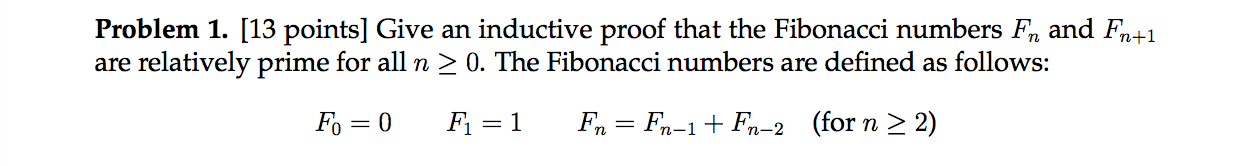
\includegraphics[width=400pt]{img/MIT-math-for-cs-2004-1.png}
\end{mdframed}

\begin{definition*}
  Integers $m$ and $n$ are relatively prime (coprime) if they have no common factors other than 1.
\end{definition*}


\begin{proof}
  $F_0 = 0$ and $F_1 = 1$ are coprime.

  Let $i > 1$ and suppose that $F_{i}$ and $F_{i+1}$ are coprime.

  We want to show that $F_{i+1}$ and $F_{i+2}$ are coprime.

  Suppose for a contradiction that $F_{i+1}$ and $F_{i+2}$ are not coprime.

  Then there exists $p, s \geq 1$ and $q > 1$ such that $F_{i+1} = pq$ and $F_{i+2} = sq$.

  Note that $F_{i+2} = sq = F_{i} + F_{i+1} = F_i + pq$, therefore $F_i = (s - p)q$, therefore
  $q$ is a factor of $F_i$, as well as of $F_{i+1}$.

  But by the inductive hypothesis, $F_{i}$ and $F_{i+1}$ are coprime, so $q$ cannot be a factor of
  both.

  This contradiction proves that $F_{i+1}$ and $F_{i+2}$ are coprime and, by induction, that the
  Fibonacci numbers $F_n$ and $F_{n+1}$ are coprime for all $n \geq 0$.


\end{proof}

\begin{mdframed}
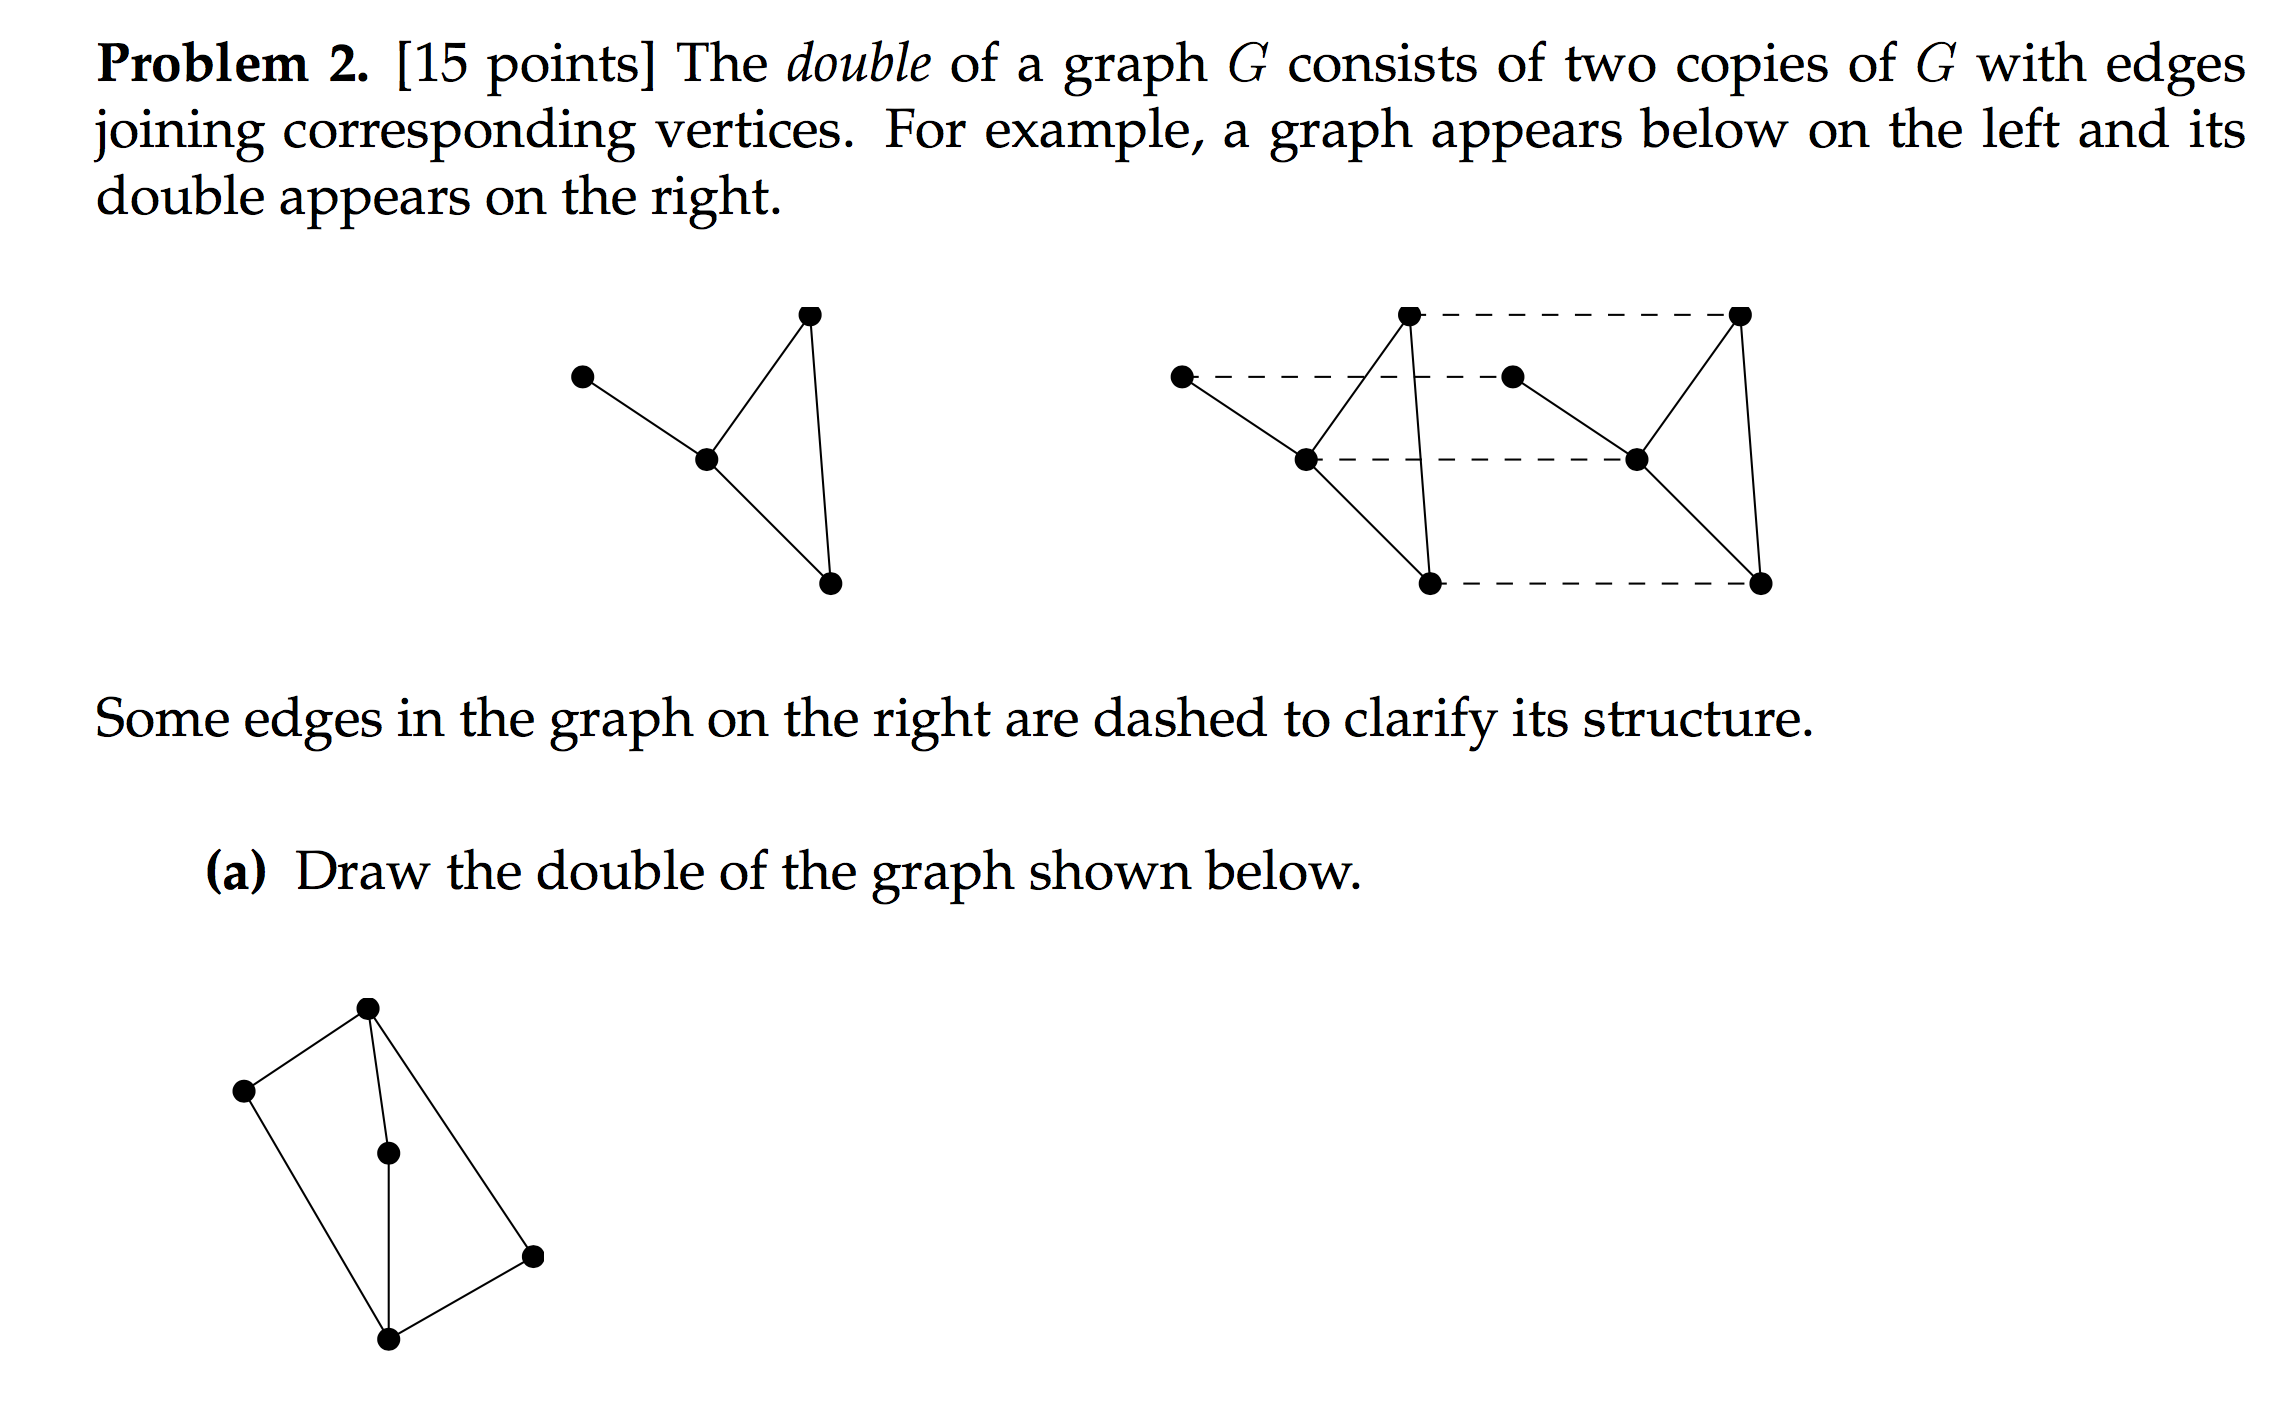
\includegraphics[width=400pt]{img/MIT-math-for-cs-2004-2-1.png}
\end{mdframed}

\begin{mdframed}
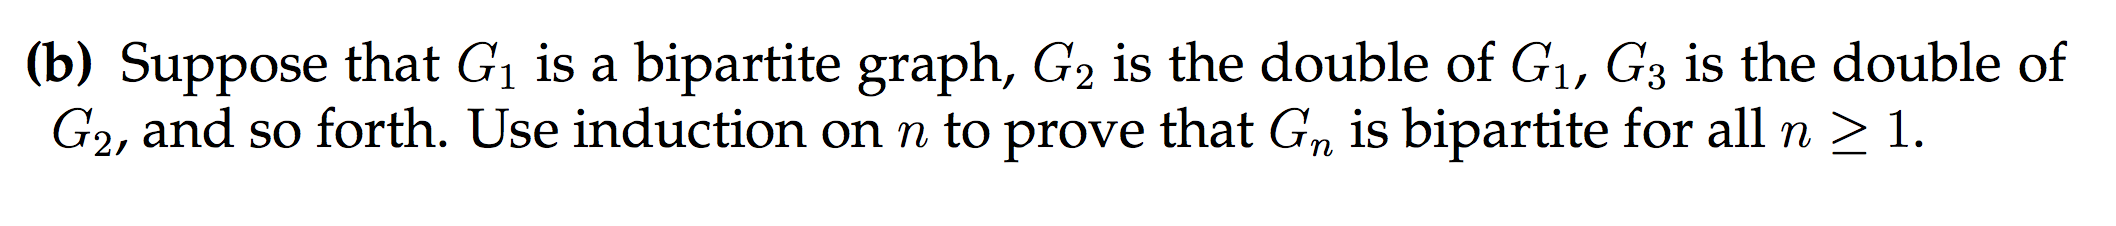
\includegraphics[width=400pt]{img/MIT-math-for-cs-2004-2-2.png}
\end{mdframed}

\begin{mdframed}
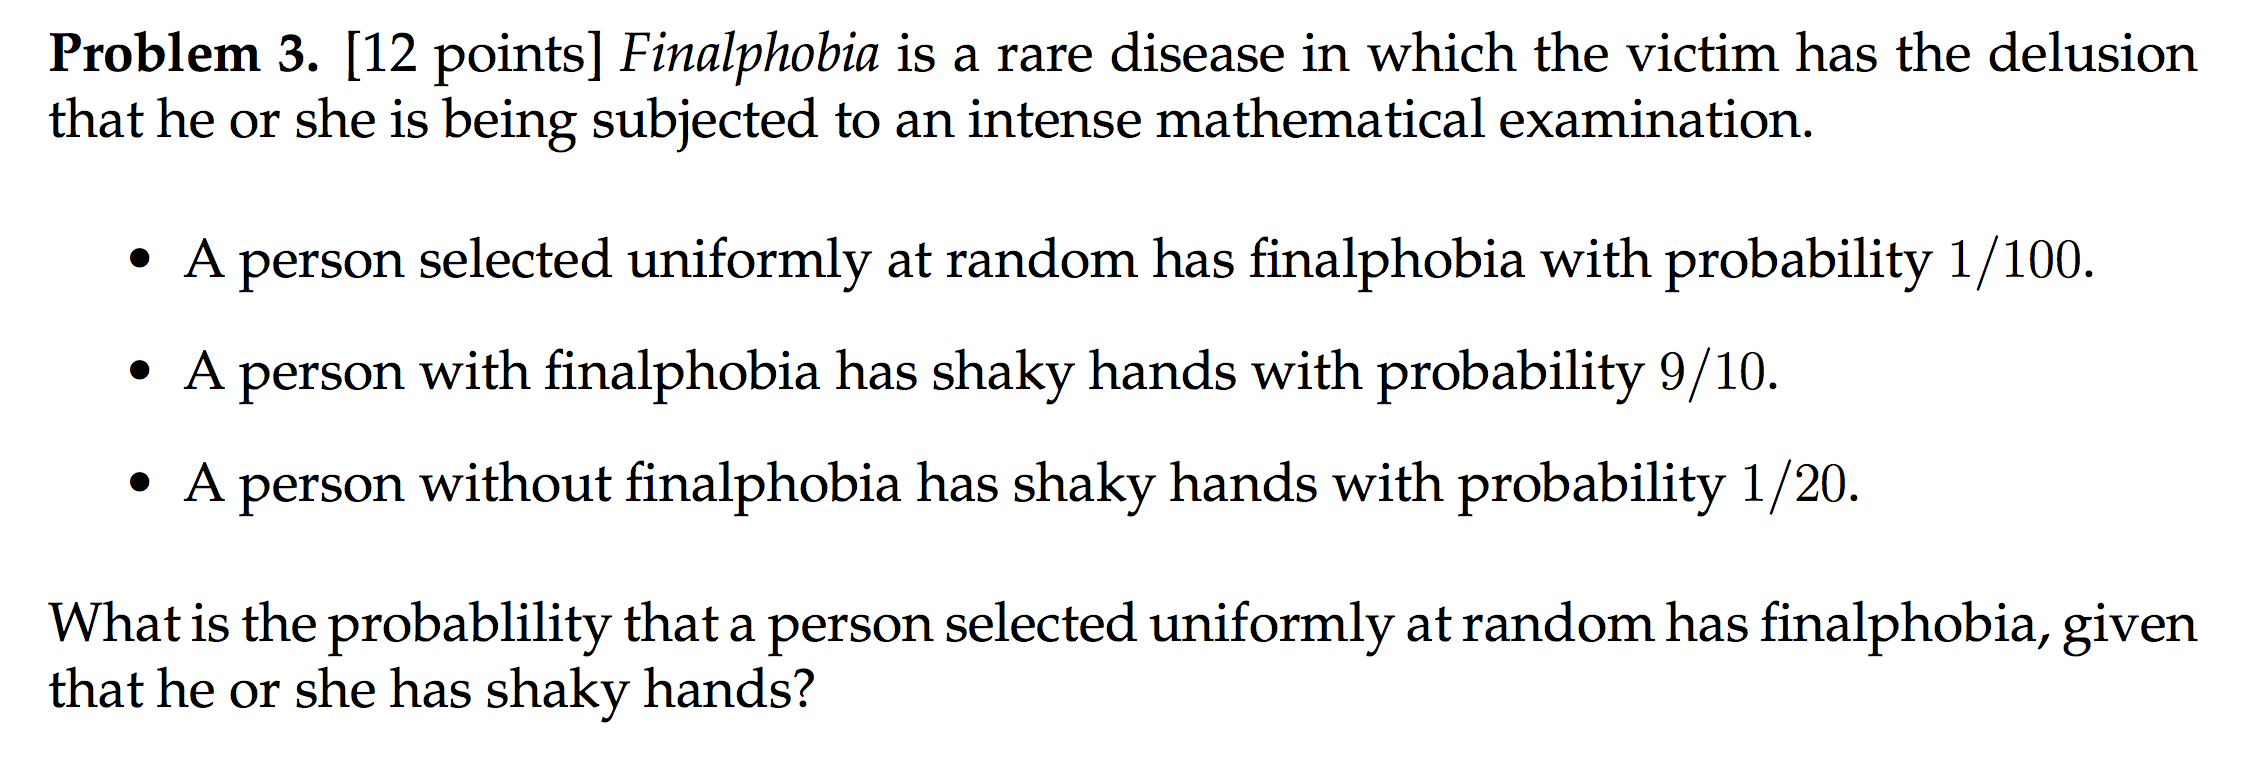
\includegraphics[width=400pt]{img/MIT-math-for-cs-2004-3.png}
\end{mdframed}

\newpage
\begin{mdframed}
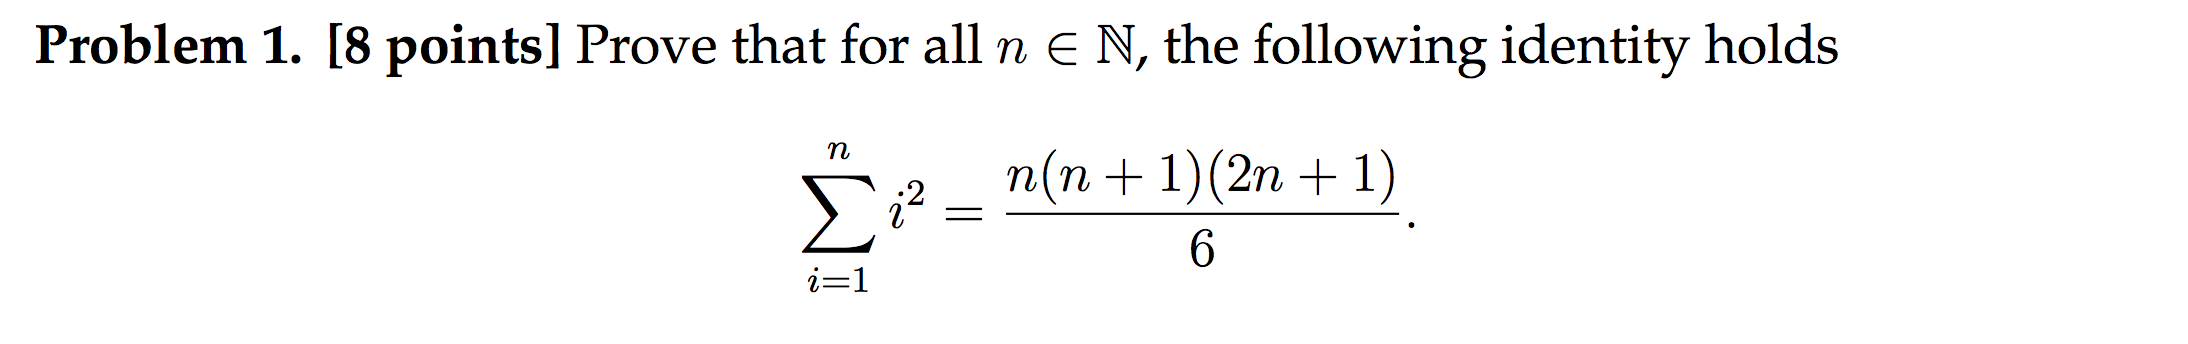
\includegraphics[width=400pt]{img/MIT-math-for-cs-2006-1.png}
\end{mdframed}
\begin{align*}
  \sumin i^2 = 1^2 + 2^2 + \ldots + n^2
\end{align*}

...induction.

\newpage
\begin{mdframed}
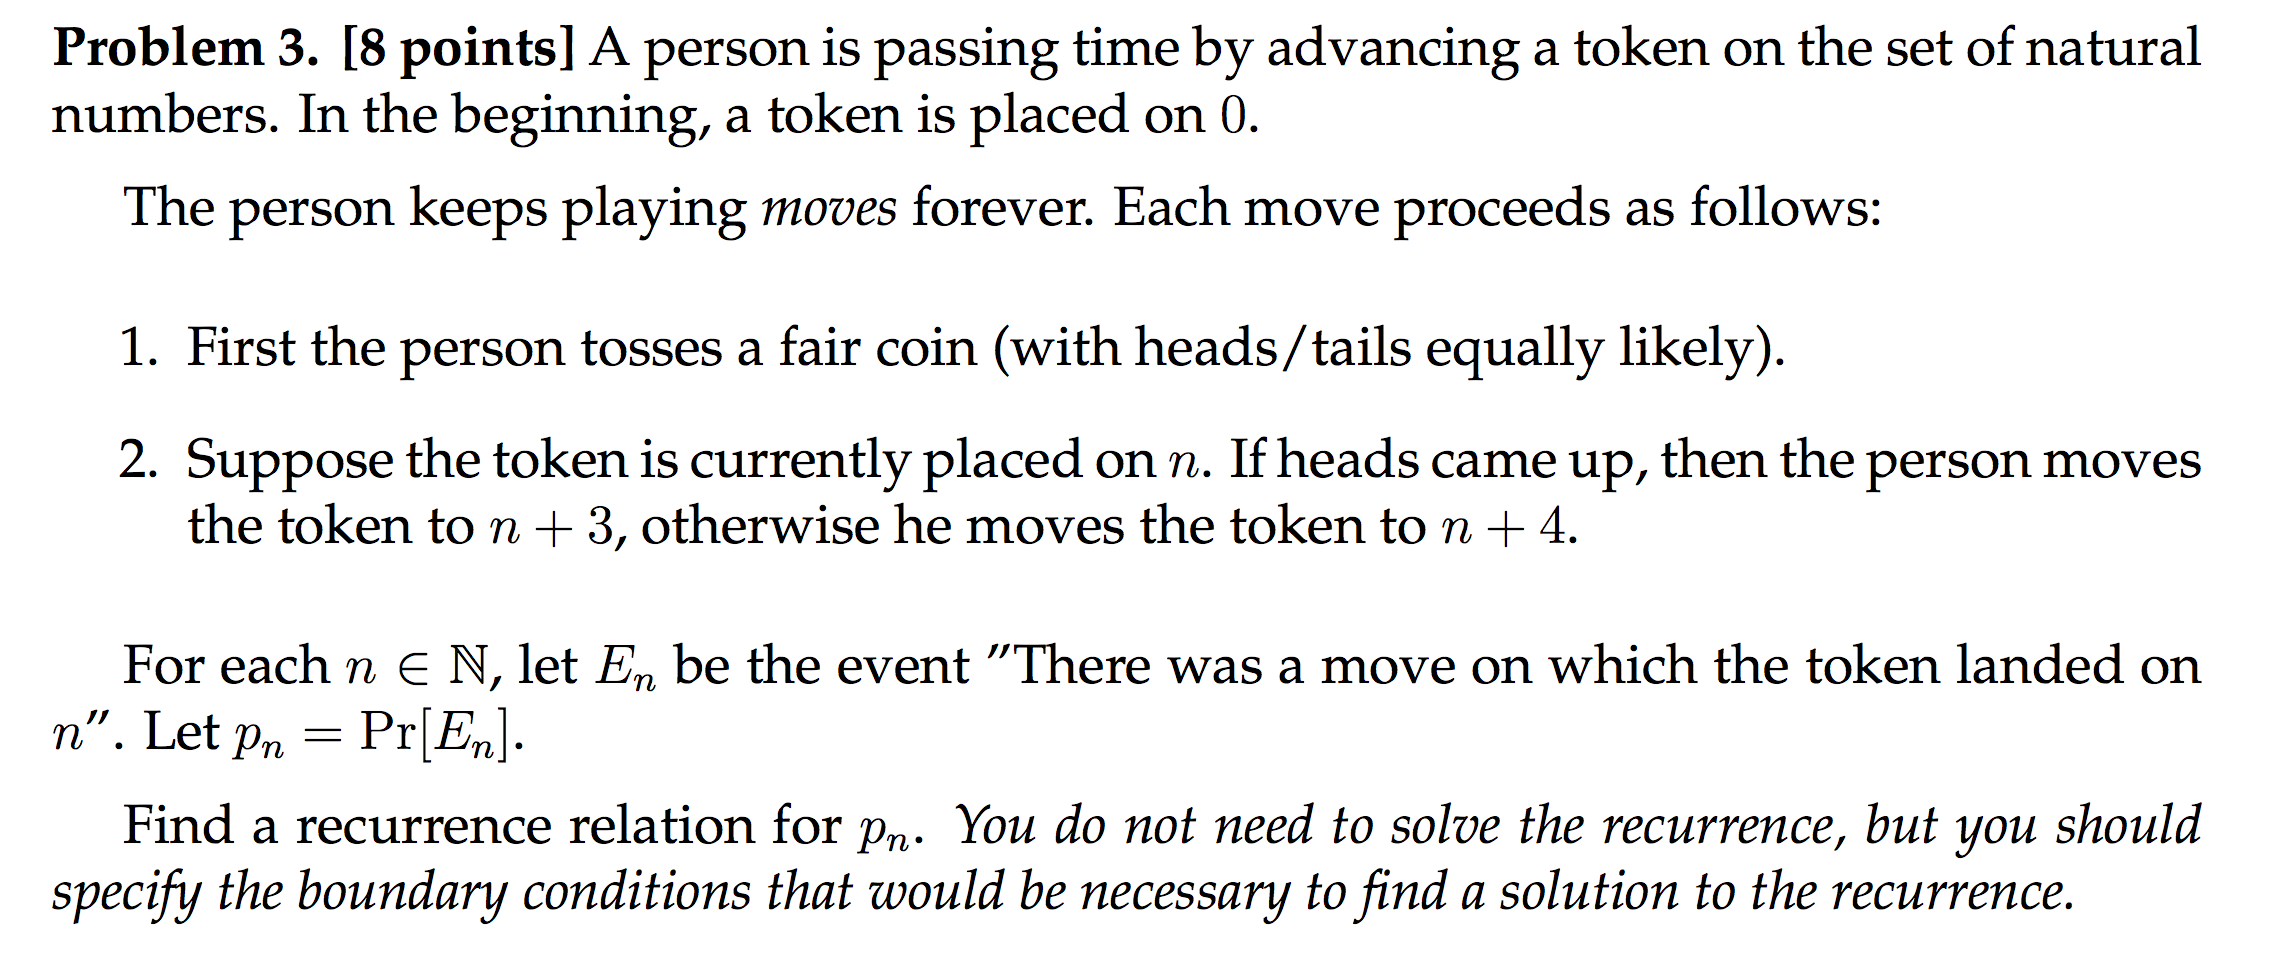
\includegraphics[width=400pt]{img/MIT-math-for-cs-2006-3.png}
\end{mdframed}
$p_0 = 1$\\
$p(1) = p(2) = 0$\\
$p(3) = \frac{1}{2}$\\
$p_n = \frac{1}{2}p_{n-3} + \frac{1}{2}p_{n-4}$ for $n \geq 4$\\

\newpage
\begin{mdframed}
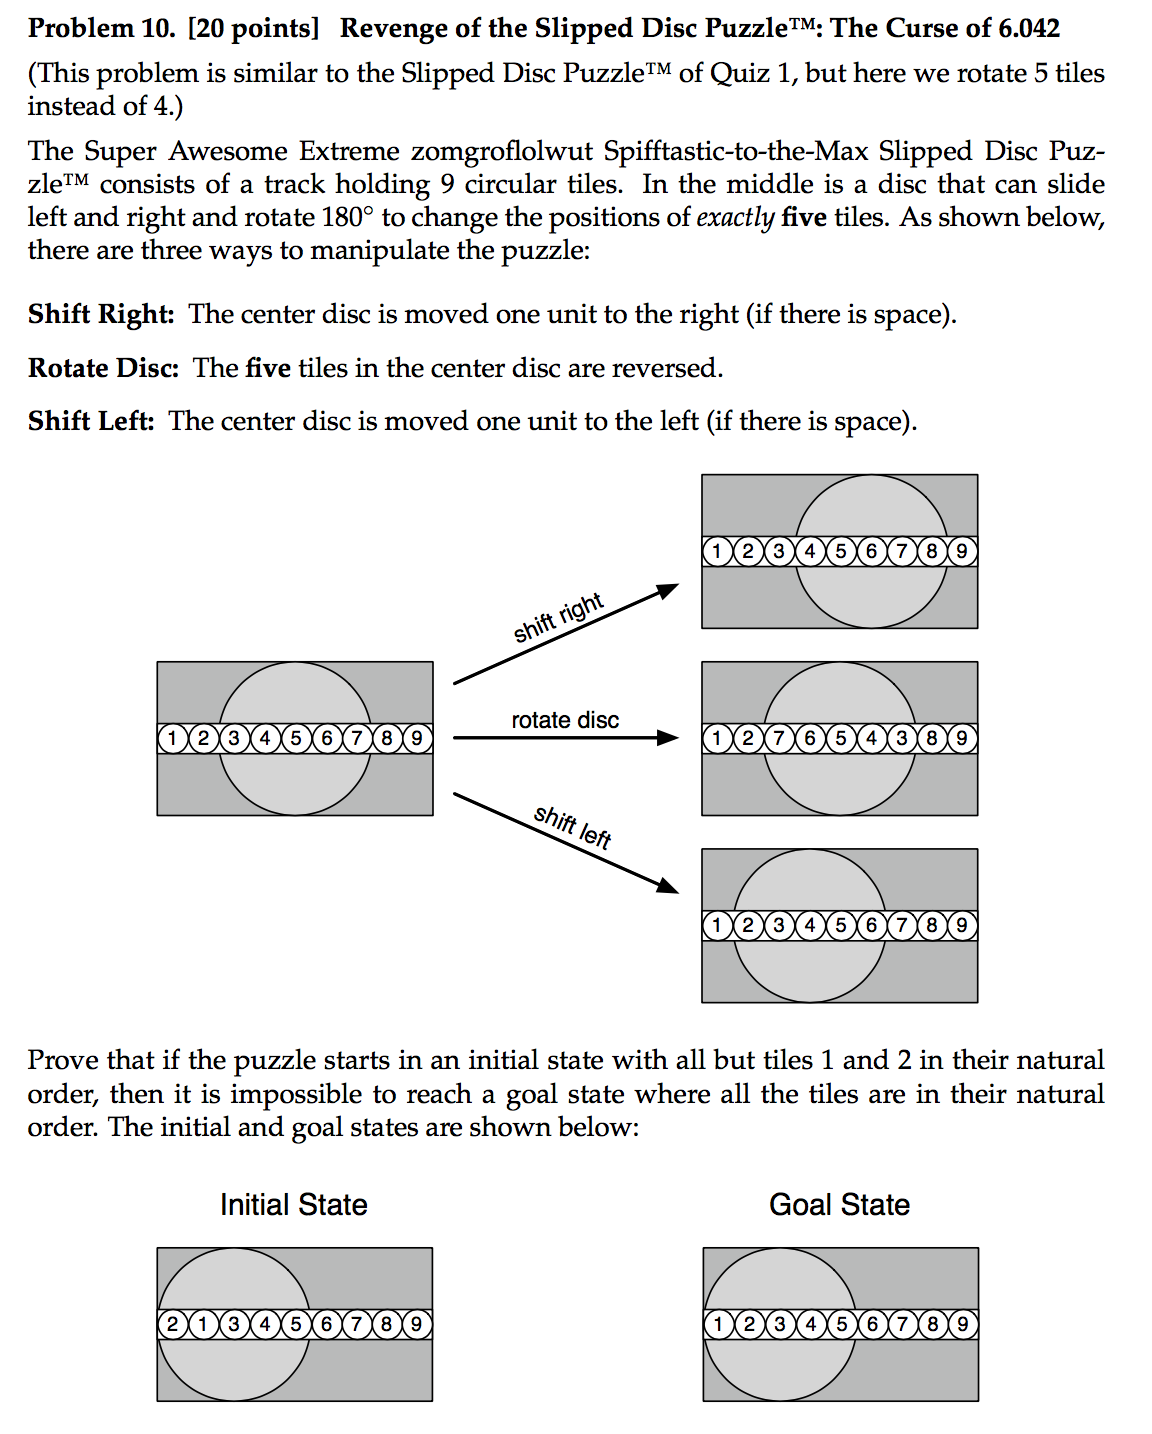
\includegraphics[width=400pt]{img/MIT-math-for-cs-2008-10.png}
\end{mdframed}

The goal is to write the permutation $(12)$ as an arbitrary composition of the following
permutations
\begin{align*}
  &(12)(45)\\
  &(23)(56)\\
  &(34)(67)\\
  &(45)(78)\\
  &(56)(89).
\end{align*}

Let's look at some compositions:
\begin{align*}
  ((12)(45))^2        &= e\\
  (12)(45) ~ (23)(56) &= (13)(46)\\
  (12)(45) ~ (34)(67) &= (12)(45)(34)(67)\\
  (34)(67) ~ (12)(45) &= (35)(67)(12)
\end{align*}


Let the positions be $1, 2, \ldots 9$.

Define the position of the dic to be the leftmost position that is under the disc. Therefore the
disc starts in position 1.

Note that every rotation affects 4 tiles and leaves 5 unchanged.

Suppose we can reach the goal state.

Then the last move is a rotation.

Note that we must perform a rotate move with the disc in position 1, since we must change the
position of the tile labeled 2 that starts in position 1.

\end{document}
